\documentclass[0main.tex]{subfiles}
\graphicspath{{./img}}

\begin{document}

\section{System implementation}

Now that the system architecture model has been designed and the technical requirements and
tools considered, it is possible to create the system implementation. In this section, the
process of building the software package and subsequent implementation into the simulator
software will be described. 

The software package design will be separated from the simulator software so that it will be 
implementation agnostic and could be used for other game engines or other simulation purposes. 

The first section will be devoted to micro-agent implementation, where it will be described which 
classes and services is the agent unit comprised of. The next section will describe how the 
communication between agents is implemented, including the implementation of the ACL and C-ITS communication 
standards and agent negotiation. 

The way the framework is built is that it mostly consists of \emph{abstract} classes that have got some 
common behavior pre-defined but require the user to specify given behavior that is exclusive to their 
use case. This allows for a framework that has got the generic behavior already completed but 
gives the user freedom and guidance concerning detailed behavior implementation. 

\subsection{Agent implementation}

As has been defined in the section \ref{sec-system} which proposed the system model, the agent component 
will be composed of the three main layers, represented as standalone classes interacting with 
each other - \emph{deliberation}, \emph{sequencer} and \emph{skill} classes.

\subsubsection{Inter-layer interaction}

There are two ways in which the individual layers can interact and inform each other. The top-down 
interaction (the deliberation layer is considered to be the top and the skill layer the bottom one) 
is done by supplying the superior (i.e. top) layer with a reference to the lower layer so that 
its whole interface is available to use. Interaction initiated by the lower layer with the upper layer 
is implemented in a different way, where the lower layer initiates a context-specific event with an 
optionally-specified content that the superior layer subscribes to. The reason behind this implementation
is that this ensures that the lower layers can't control the upper layers but rather just inform them about 
potentially important/interesting events that have taken place while operating and interacting with 
the environment.

Below is a class diagram of the components with marked dependencies, including their methods and 
properties (fig. \ref{mas-its-components}).


\begin{figure}[htbp]
    \centering
    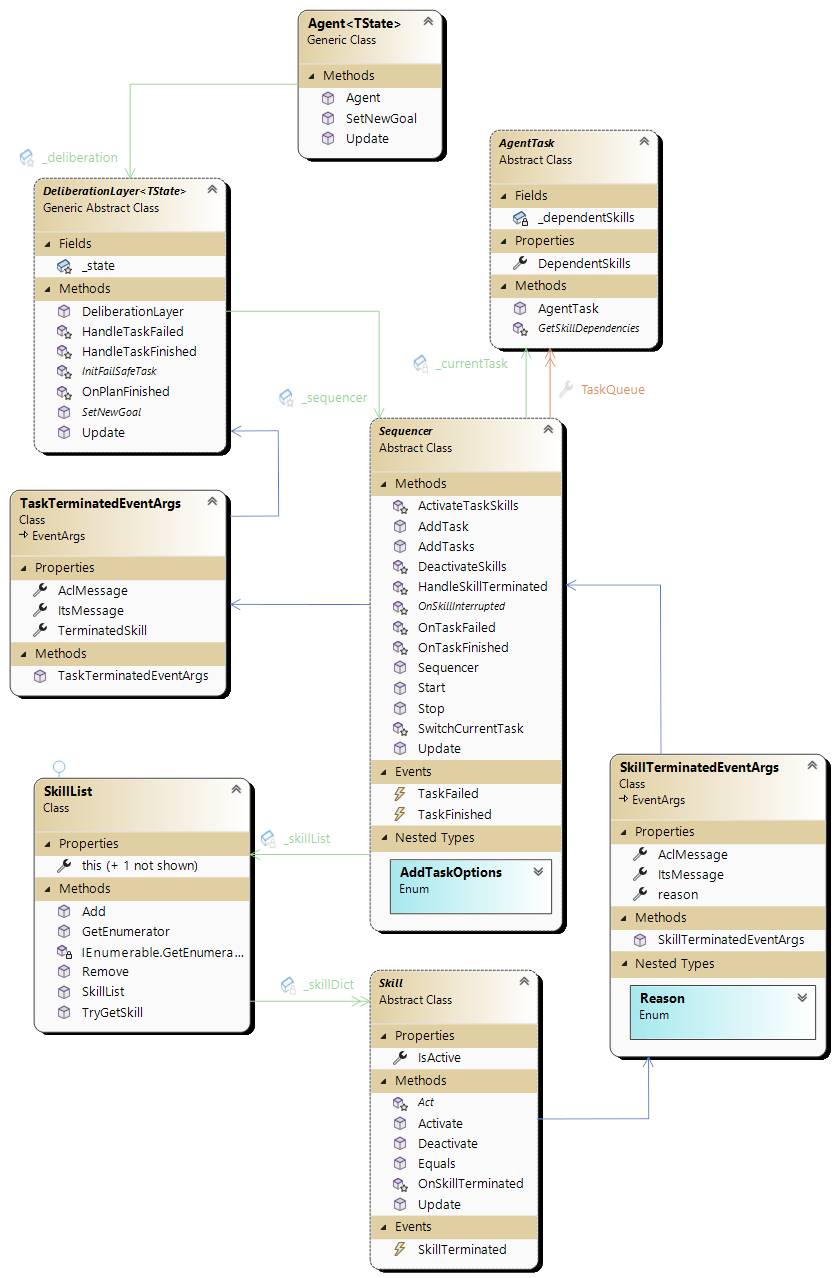
\includegraphics[width=.9\textwidth]{MAS-ITS-Components.png}
    \caption{Class diagram of main agent framework components}
    \label{mas-its-components}
\end{figure}

\subsubsection{Deliberation layer}

The deliberation layer is the highest from a hierarchical point of view. Its responsibility is to 
create a plan that satisfies a goal that the agent gets as input. Apart from the layer 
being abstract (i.e. requiring further implementation details specified by inheriting from the 
class), it is also generic, which means that it will defer the type specification of its state until 
it is declared by the derived class. This leaves the state specification to be implemented 
to the user's needs. For example, a vehicle agent can have its state as a three-dimensional
vector, whereas a broadcasting station will have its state defined as one of its possible
states (e.g. represented by a single discrete number).  The initial value of the state parameter
is required to be specified upon object instantiation/creation.

Upon providing a goal to the layer by the executing client, it should resolve it by
initializing a sequence of pre-defined \texttt{AgentTask} objects whose execution should 
accomplish the goal. The input goal should be defined 
as a high-level keyword, and the layer is assumed to receive only pre-defined goal keywords,
which will be matched to different patterns of task-resolving logic.

The \texttt{AgentTask} class encapsulates a list of skill types that shall be activated 
once the task is executed. The skill list does not contain the actual instantiated 
objects, but just information about skill type (derived from the \texttt{Skill} abstract 
class). Such type of pseudo-contract is then transferred to the \texttt{Sequencer} layer and 
validated at run-time. In other words, the \texttt{Sequencer} class must contain instantiated
\texttt{Skill} objects listed in the received \texttt{AgentTask}.

To offer a form of task reuse, a parametrization of tasks is implemented. This feature is 
implemented in a way that the task also contains an optional transform procedure delegate which 
gets passed to the \texttt{Skill} object once it's activated as part of the task execution.
As an example, a task that contains a general communication skill that broadcasts messages to
other agents can have the broadcasted message type and content specified differently in each 
separate instance of resolved tasks. The logic in the \texttt{AgentTask} type can be reused 
while allowing for parametrized Skill initialization (e.g. broadcasted information type). 

This layer can also receive notification from the lower layer when a task has failed or 
the initialized sequence of tasks (i.e. plan) has finished. As defined in the system requirements, 
the user must implement behavior when the execution of an instantiated plan has failed or 
has been interrupted by impacting events in the operating environment. The user has to implement 
a fail-safe \texttt{AgentTask} that will get activated in case the Deliberation layer is not able 
to achieve the specified goal. 

\subsubsection{Sequencer layer}

The \texttt{Sequencer} class is responsible for the most amount of general logic. This is because 
it interacts with both the upper and lower layer and hands over information about skill execution 
to the Deliberation layer. Its primary responsibility is to keep track of currently executing skills 
and activate or deactivate them respectively to the currently executing task. 

When the Deliberation layer generates a sequence of tasks, it is enqueued into the
\texttt{Sequencer}'s internal task queue. The tasks in the queue get sequentially executed. 
Before activating skills according to the task specification, the task-specific 
initialization transform, if there is any, is applied to respective Skill(s). Afterward, 
the Skills get activated by the Sequencer. The \texttt{Sequencer} class also exposes the interface 
to the upper (Deliberation) layer to dynamically add to or overwrite the \texttt{AgentTask} queue 
during runtime. This can come useful when there are immediate changes to the environment which 
the Deliberation layer evaluates to re-plan to reach the current goal. 

Another responsibility of the \texttt{Sequencer} class, which requires implementation from the 
user by inheriting from the base class, is Skill termination management. The class gets notified about skill terminating
by subscribing to the \texttt{SkillTerminated} event for each of the Skills bound to the layer.
When one of the Skills triggers such an event and terminates, the \texttt{Sequencer} gets information 
about the \emph{type} of terminated Skill and \emph{termination reason}, which is of one of 
three defined values - \texttt{Finished}, \texttt{Interrupted} or \texttt{Failed}. The logic 
implemented by the user, based on the type- and reason-based inputs, should identify whether 
the case of Skill termination is detrimental to the execution of the whole task (meaning 
task execution has \emph{failed} or \emph{finished}). If so, the \texttt{Sequencer} triggers
the respective task termination event and the resolving logic is handled to the \texttt{Deliberation}
class. Alternatively, the terminated Skill can be left disabled or re-started. 

\subsubsection{Skill layer}

The Skill layer comprises a defined collection of objects derived from the base
\texttt{Skill} class. The implementation of the base abstract class is only about 
defining its methods that should ensure proper integration with the upper layers, such 
as methods for activation and deactivation of the skill exposed to the \texttt{Sequencer}
class.

The implementation required by the user-specific use case of a particular skill is mainly 
the \texttt{Act} method implementation, where the user is required to specify the Skill's
computational transform (as specified by the requirements in section \ref{sec-system}).

The Skill layer is also expected to utilize the chaining of Skill inputs and outputs. Skills are 
expected to slightly vary in abstraction level, meaning there should be Skills directly 
interacting with the agent's sensory hardware and providing such information as an output. 
The logic which makes use of the agent's sensors to compute additional transform should be encapsulated in
a dedicated Skill to conform with each Skill having a single responsibility. Skill chaining 
is defined in the class derived from \texttt{Skill}. Skill outputs are defined as 
public class properties. To allow the use of Skill \texttt{A}'s output in skill \texttt{B},
the reference of \texttt{A} is provided in \texttt{B}'s constructor. The \texttt{B} Skill 
can then use \texttt{A}'s exposed output property in its transform function.

An activity diagram sowing process logic and interaction between inner components can be 
seen in figure \ref{fig-activity-diagram}.

\begin{figure}[htbp]
    \centering
    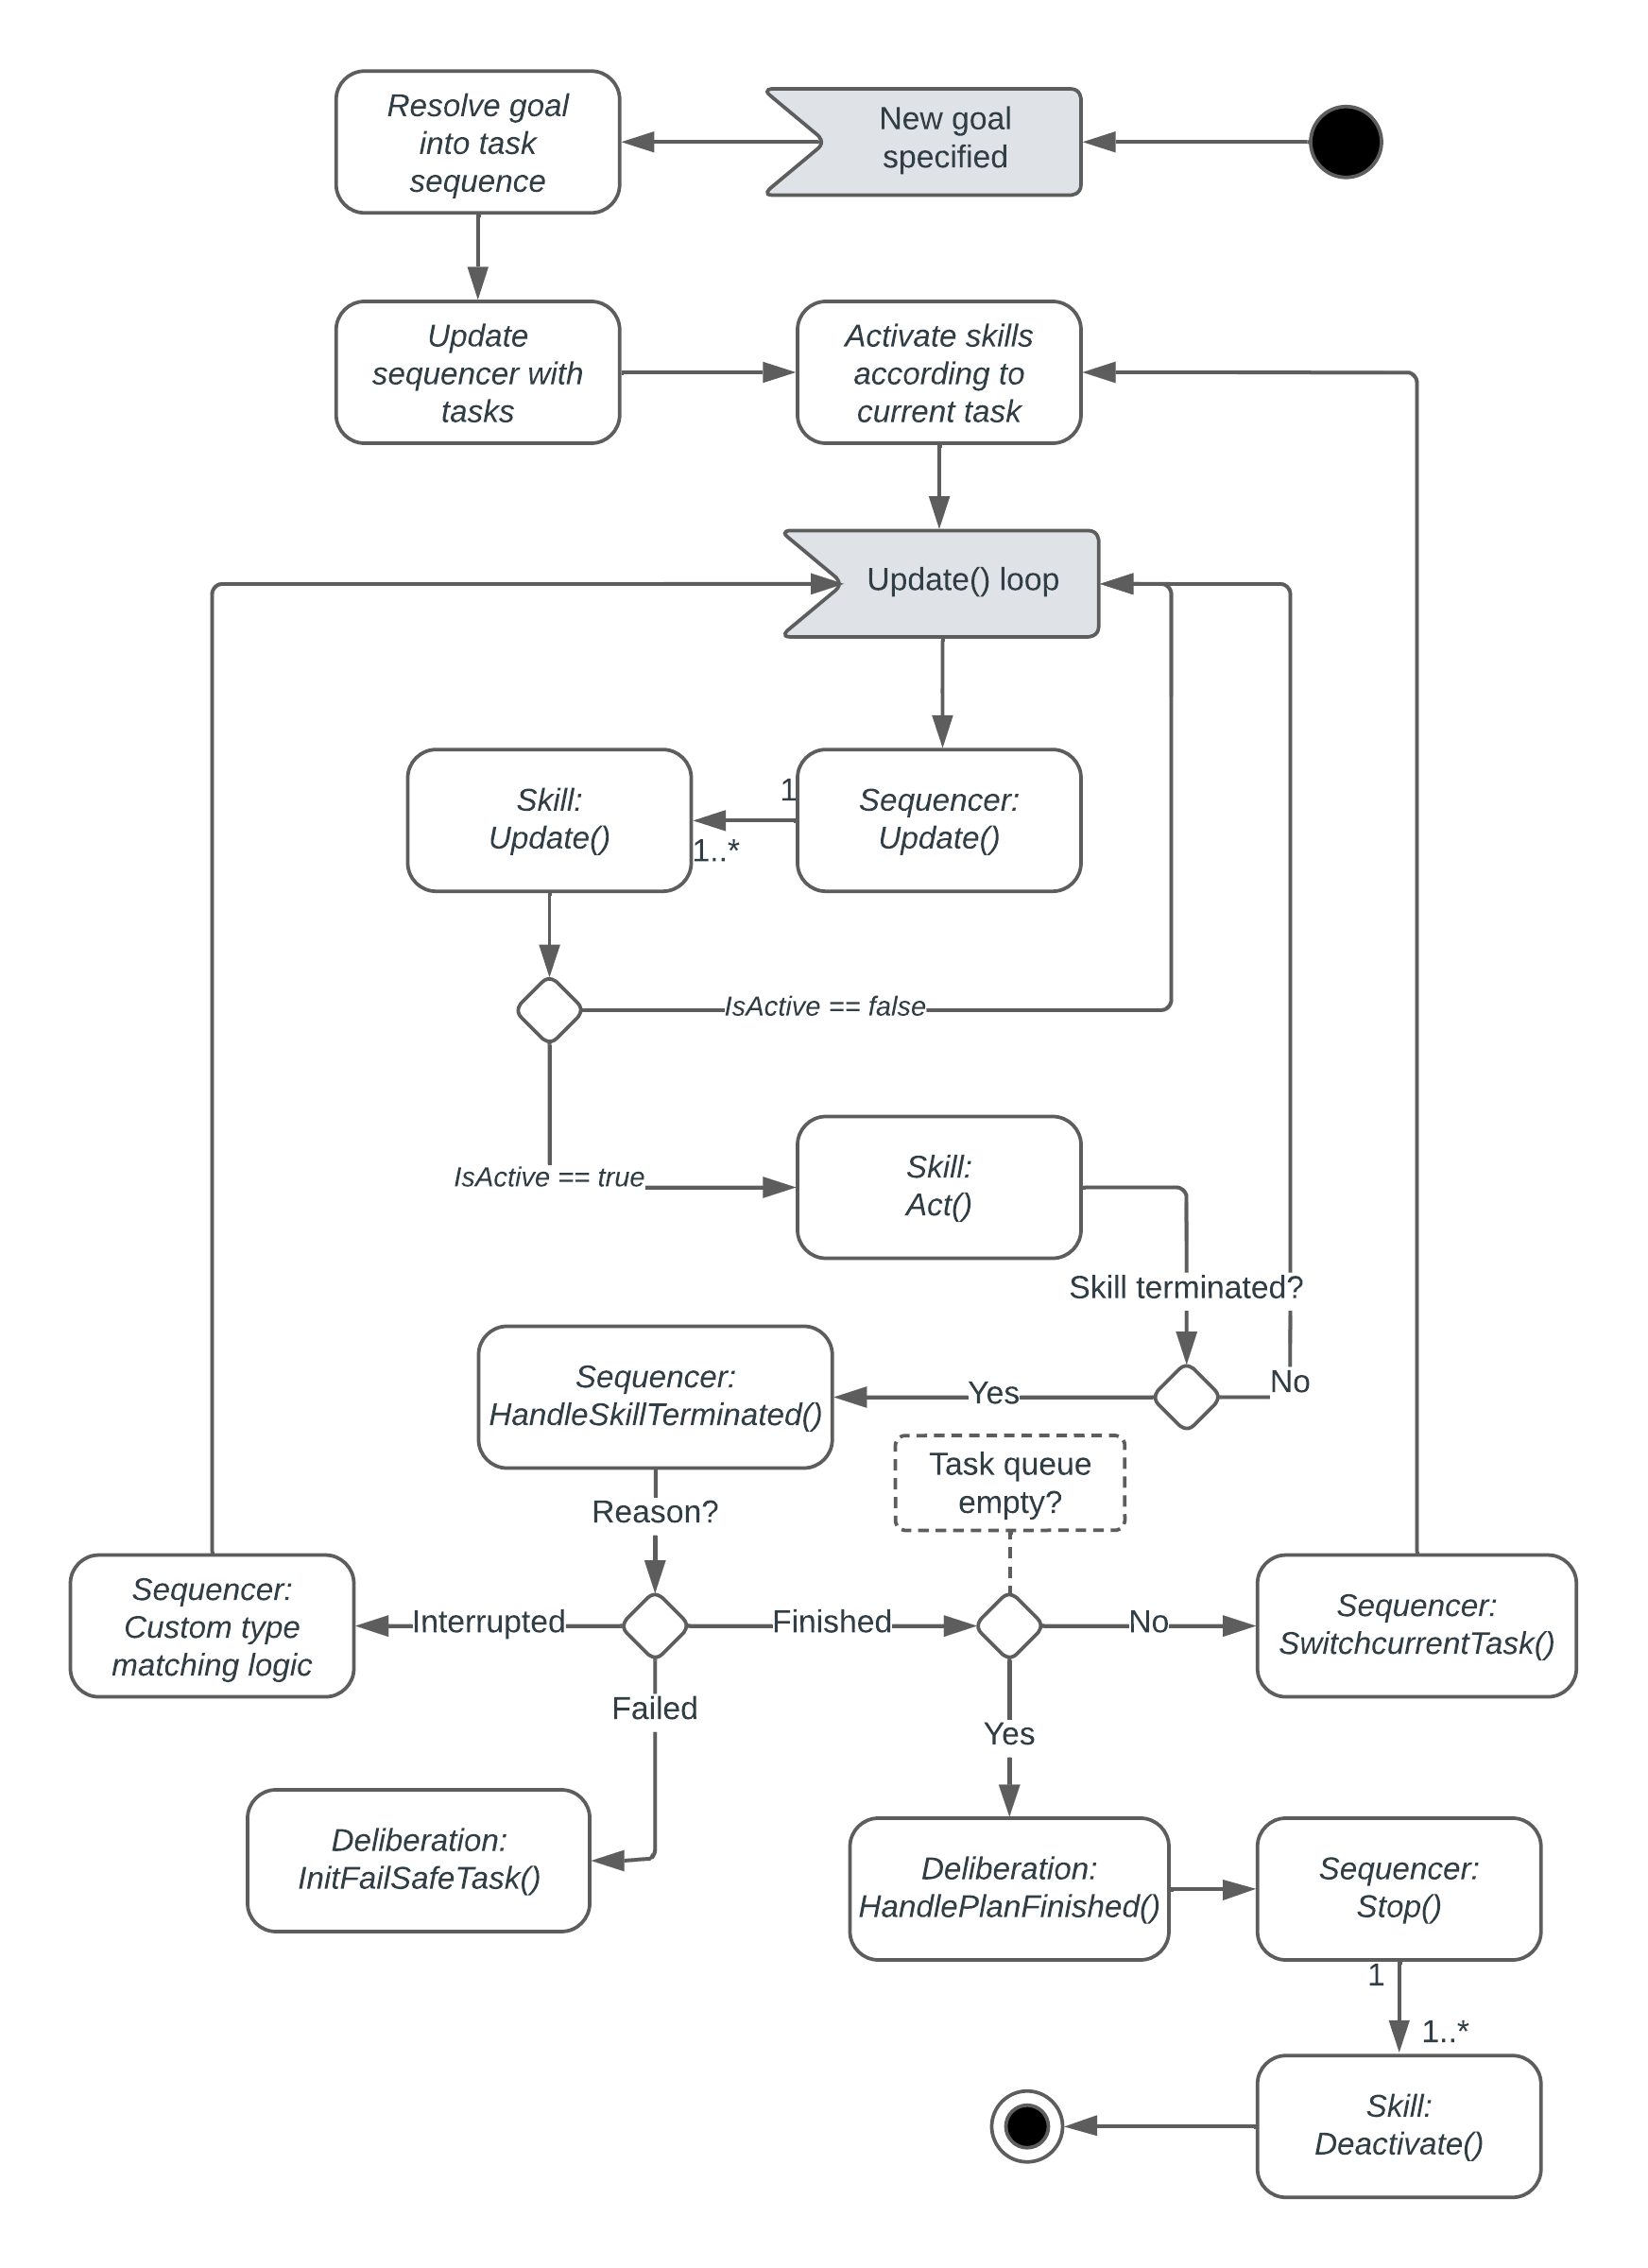
\includegraphics[width=.9\textwidth]{3T-Activity-diagram.png}
    \caption{Trivial activity diagram of the implemented \textsubscript{3}T architecture}
    \label{fig-activity-diagram}
\end{figure}

\subsection{Communication module implementation}

As has been started section \ref{sec-requirements}, where in the system requirements were
defined, the framework will come with a pre-implemented communication interface which will 
allow the agents to exchange pre-defined messages. There are two
base object types handling communication between agents - an agent-bound
\texttt{CommunicationSkill} class that serves as an agent's proxy to the communication space,
and the \texttt{MessageBroker} class that handles message delivery to individual agents. In
addition to that Message types created according to the C-ITS and ACL standards were created to
carry appropriate content. The class diagram of the communication interface can be seen in
figure \ref{fig-classes-comm}.

\subsubsection{Message broker}

The \texttt{MessageBroker} is a \emph{static} class (only one allowed instance per 
simulation) which manages message delivery and simulates the communication space. 
It manages both the ACL and C-ITS messages by providing overloads for its methods 
based on the provided message type. Because the class is static, agents\footnote{More precisely,
communication skills that agents come equipped with} can interact with it without 
having to hold a reference to it. Agents can:

\begin{itemize}
    \item Register to message broadcasts
    \item Broadcast messages themselves 
    \item Send messages directly to specific agents
\end{itemize}

When an agent registers to the class, it holds its reference in its register. 
That way the class can access the registered agent's inbox when a message is 
being delivered.

When sending/broadcasting a message, apart from providing the actual content (i.e. 
the message object), the message must be "wrapped" in a \texttt{tuple} which must 
contain the sender ID. When sending the message directly, obviously, the sender must 
provide the recipient agent ID. 

\subsubsection{Communication Skill}

The \texttt{CommunicationSkill} class derives from the base \texttt{Skill} class, so it should
be handled like any other skill. This type itself is \emph{generic} and \emph{abstract}. For
the skill to be used, a derived class with a specified Message type needs to be created and
implemented. The pre-defined behavior is in the \texttt{Act} method, where all Messages to
broadcast are handed to the \texttt{MessageBroker} class.  The Messages to broadcast are
specified upon \texttt{AgentTask} initialization by the transform procedure. That way,
different \texttt{AgentTasks} can re-use the single \texttt{CommunicationSkill} class.  Then,
all messages received in the Skill's \texttt{ReceivedMessagesQueue} are processed. The message
processing logic should be implemented by the user by pattern matching. The pattern matching
can be defined in the \texttt{CommunicationSkill} itself, but to honor the single
responsibility paradigm, a better way is to use the pre-defined behavior, where a
\texttt{MessageReceived} event is invoked and other Skills subscribed to this event can process
the message, deciding if they are interested in the contents and acting upon it accordingly. 

\subsubsection{Message implementation}

%% TODO: image reference %%
The ACL and C-ITS (i.e. DENM and CAM services) message contents were implemented according to 
the official documentation. For reference, the ACL message contents can be seen in the figure
\ref{message-structure} and table \ref{cas}, the C-ITS message contents can be seen 
in figures \ref{cam-spec} and \ref{denm-spec}.

\begin{figure}[htbp]
    \centering
    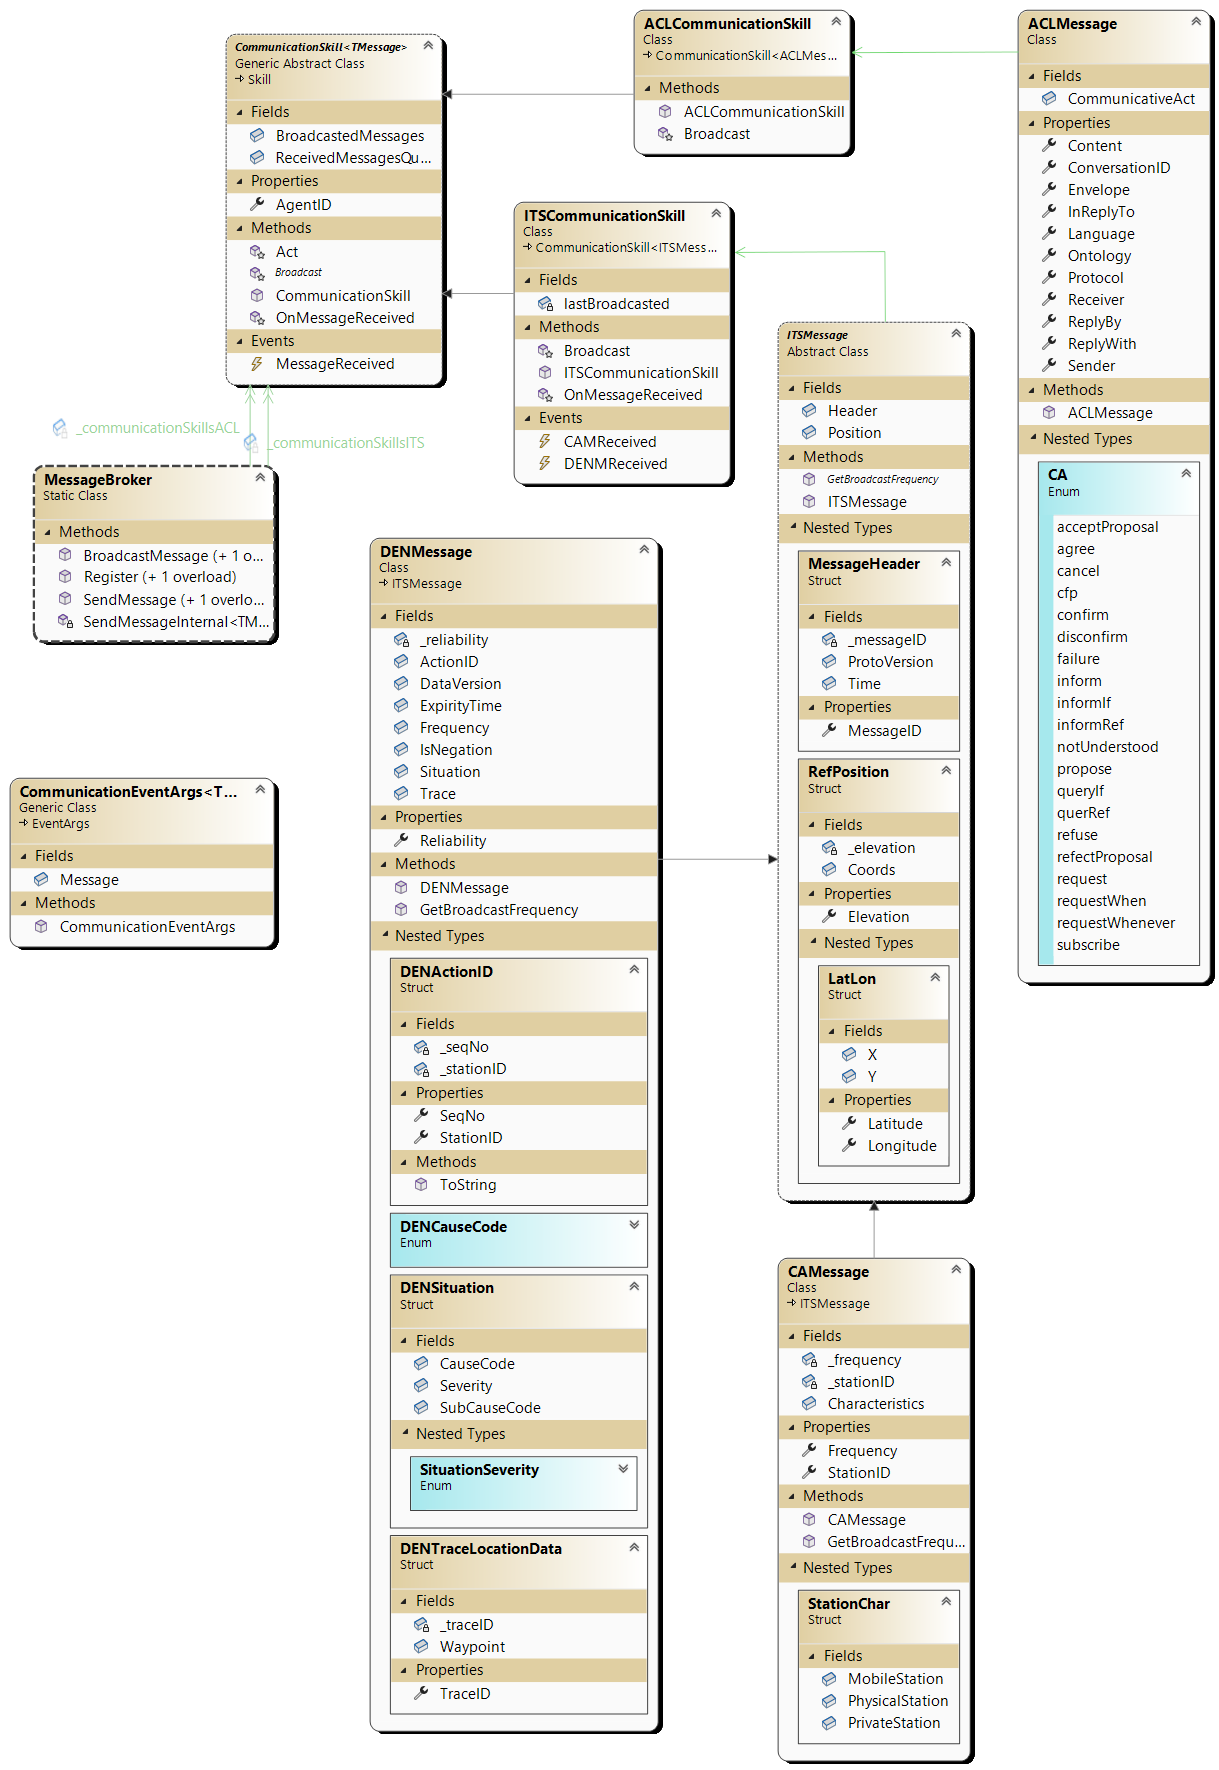
\includegraphics[width=.99\textwidth]{mas-its-communication.png}
    \caption{Class diagram of the implemented communication interface}
    \label{fig-classes-comm}
\end{figure}

\subsection{Unity integration}

As has been mentioned in the introduction to Unity software in the section \ref{sec-toolset}, programmatically 
defined behavior is implemented by assigning C\# scripts as individual components to game objects in 
the scene. The scripts are not being executed by a main client script like in conventional software, but 
rather by calling an \texttt{Update} method in the Unity script which is invoked by the Unity engine 
on each game tick. Such behavior is obtained by inheriting from the \texttt{MonoBehaviour} class, which 
also defines other methods that get invoked in certain scenarios. Including the \texttt{Update}
method, the standard methods used in most cases are:

\begin{itemize}
    \item \texttt{Start} method, which substitutes object initialization 
through the constructor and is called at the start of the script lifetime
    \item \texttt{OnDisable} method, which gets called when the script component or the whole game object 
    gets disabled. Disabled components aren't rendered and cannot interact with the scene nor be interacted 
    with. 
    \item \texttt{OnEnable} method, which is inverse to the previous and gets called when game objects 
    or components are enabled/activated.
\end{itemize}

The idea behind the proposed MAS ITS framework integration with Unity is to assign the \texttt{Agent} 
class to game objects as a component in order to use the game object as an agent. For instance, the game object can be 
a vehicle model or even a non-physical game object invisible in the scene, for example, a traffic controller. When 
the \texttt{Agent} class would get assigned to a game object, it would be able to interact with its other game
components and object properties through pre-defined sensor or actuator skills. 

Although the \texttt{Agent} class and its components (i.e. layers) come with the \texttt{Update} method in 
their default implementation, it will still not get called by the Unity engine. For that reason, a \emph{wrapper}
class \texttt{AgentMonoWrapper} been created. This class will get added as a component to the game object that 
the user wants to induce agent behavior on. The class will initialize an agent by calling an abstract method 
\texttt{InitAgent()} at \texttt{MonoBehaviour.Start()} invocation and call \texttt{Agent.Update()} on 
\texttt{MonoBehaviour.Update()} invocation. 

\subsection{Conclusion}

In this section, the implementation details of the proposed framework were discussed. The C\# language has been 
used to write the framework's code, as per the discussion in the section \ref{sec-toolset}. The framework's core 
components were defined as abstract classes, implementing general behavior and defining required behavior to 
be implemented by the user, which is use-case dependent. For instance, such behavior can be the \texttt{Act}
method in the \texttt{Skill} layer, which serves as Skill's way of interacting with the environment, which is 
different for every defined Skill. The relations between classes and inner processes have been described, serving 
as documentation for the usage of the framework. 

As per the initial requirements, the agent interaction interface has been implemented. The framework's agent 
architecture components have been used to create dedicated communication skills that can broadcast and 
directly send standardized messages to each other together with a custom messaging service.
Consequentially, a C\# implementation of ACL and C-ITS (CAM, DENM) message standards has been created to
be used in the framework. 

Lastly, integration of the framework with the Unity game engine has been discussed and described in detail, 
introducing an additional wrapper component to ensure proper cross-interaction.

\clearpage

\end{document}